\documentclass{article}


\usepackage{graphicx}
\usepackage{amsmath}
\usepackage{natbib}
\title{poissonNMF -- blind source separation of fluorescence microscopy data}
%\author{Richard Neher, Andr\'e Zeug and Fabian Theiss}
\newcommand{\bm}[1]{\mbox{\boldmath $#1$}}
\newcommand{\EQ}[1]{Eq.~(\ref{eq:#1})}
\newcommand{\EQS}[2]{Eqs.~(\ref{eq:#1)} and (\ref{eq:#2})}
\newcommand{\FIG}[1]{Fig.~\ref{fig:#1}}
\newcommand{\REF}[1]{ref.~\citep{#1}}

\bibliographystyle{unsrtnat}
\begin{document}
\maketitle
PoissonNMF is an ImageJ plugin to decompose spectrally resolved fluorescence
microscopy data into the contribution of the labels under conditions where the
spectra are not or only inaccurately known. It employs non-negative matrix
factorization \cite{Lee_Nature_99}, suitably modified to shot-noise dominated
data \cite{Neher_BPJ_2009}. 

\section*{Installation}
To install the plugin, copy the \texttt{PNMF\_.class} and 
\texttt{PNMF\_\$1.class} files as well as the into folder
\texttt{PNMF\_SpectraLibrary} the plugins directory of your ImageJ
distribution. 

\section*{Input Data} PoissonNMF expects a 32 bit image stack, where each 
slice of the stack corresponds to the image in one spectral channel. 

\section*{Parameters \& initial conditions} Upon invoking pNMF from the plugin
menu, a dialog opens, prompting the user for the number of sources expected in
the sample. This dialog is followed by a second dialog allowing the user to
provide additional input. The dialog is preset to the values of the previous
run of PoissonNMF. The dialog is shown in \FIG{dialog}. Several choices in this
dialog invoke additional dialog after the \emph{Run} button has been pressed. 
% \usepackage{graphics} is needed for \includegraphics
\begin{figure}[htp]
\begin{center}
  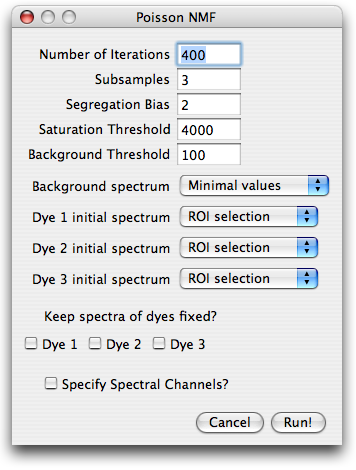
\includegraphics[width=0.8\columnwidth]{parameterDialog}
  \caption{The parameter dialog of pNMF with default values.}
  \label{fig:dialog}
\end{center}
\end{figure}
\subsection*{Parameter Dialog}
\paragraph{First and last wavelength:}

\paragraph{Number of iterations:} 
The total number of iterations the algorithm is run. Depending on the
subsampling scheme (see below), the first iteration are only applied to a
subset of the data. 
\paragraph{Subsampling:}To speed up the calculation, the algorithm can be
initiated on a subset of the data and then successively uses the estimate for
the spectra for larger subsets of the data. The parameter subsampling
determines the number of subsamplings of increasing size to be made. Successive
subsamples are larger by a factor of 10, while the last is the entire data set
(above the background threshold). The number of iterations for larger subsamples
is smaller (a factor 2 between successive subsamples).
\paragraph{Segregation Bias: } A parameter determining the degree,
to which overlap of estimated label distribution is penalized. Suitable weights
of the segregation bias are around 1 or lower. Too high segregation bias will
yield in a faulty decomposition.
\paragraph{Saturation threshold:}Saturated or nearly saturated pixels have
distorted emission spectra and therefore have to be excluded from the
analysis. If the signal in any channel at a certain pixel is above this
parameter value, the pixel is excluded. 
\paragraph{Background threshold:}Very faint pixels carry little information
and are likely dominated by noise, autofluorescence and the like. It is
therefore advisable to limit the spectra estimation to reasonably strong
pixels. Any pixel, where, after background subtraction, the intensity is below
this threshold in every channel is therefore excluded. 
\paragraph{Background:}Any constant background has to be subtracted before the
image is processed. This background is either estimated using the minimal value
in each spectral channel. Alternatively, the background can be estimated by
specifying a ROI that contains nothing but background signal or the background
can be entered manually.
\paragraph{Start spectra:}Convergence is faster if the initial spectra are
good guesses of the actual spectra. PoissonNMF provides several options to
specify the start spectrum for each dye, which can be chosen from a
pull-down menu. The simplest choice for the initial spectra are equally spaced
Gaussians. Other options to specify start spectra are ROI selection, manual
entry of the spectra and the choice of spectra from the spectra library.
\paragraph{Fix Spectra:}The initial spectrum of each dye can be kept fixed
during the PoissonNMF run by checking the appropriate checkbox. 
\paragraph{Channel boundaries:}To display the spectra correctly and to read
spectra from the library, the boundaries of the spectral channels have to be
entered. To do so, check the check box and you will be prompted for the channel
boundaries later. 

\begin{figure}[htp]
\begin{center}
  \includegraphics[width=0.7\columnwidth]{spectraSelection}
  \caption{The user is asked to specify the background and the initial spectra
  for the run of PoissonNMF.}
  \label{fig:spectraSelection}
\end{center}
\end{figure}


While PoissonNMF processes the image, the current spectra are continuously
displayed. At any point, the user can cancel the PoissonNMF or use the current
spectra for least squares unmixing of the image. 


\section*{Output}
PoissonNMF displays an image stack with the estimated label
distributions and opens a window with a number of buttons that allow to save
the spectra, examine the background spectrum and the set of background pixels
and construct RGB overlays of a triplet of dye distributions. 

\begin{figure}[htp]
\begin{center}
  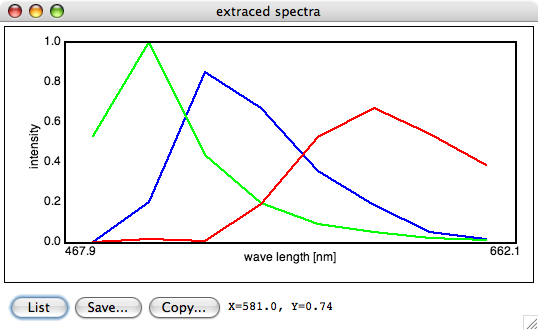
\includegraphics[width=0.8\columnwidth]{spectra}
  \caption{An example estimated spectra delivered by PoissonNMF.}
  \label{fig:spectra}
\end{center}
\end{figure}
\begin{figure}[htp]
\begin{center}
  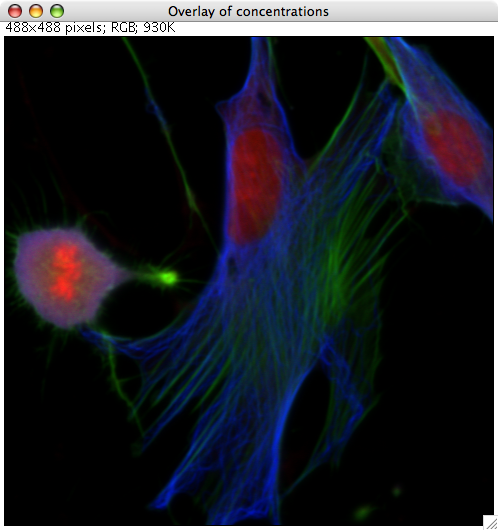
\includegraphics[width=0.9\columnwidth]{RGBoverlay}
  \caption{For three sources, PoissonNMF calculates a composite image with
  each source specifying one color channel. }
  \label{fig:RGBoverlay}
\end{center}
\end{figure}


\section*{Spectra Library}
PoissonNMF can make use of literature spectra or spectra determined in previous
runs, for example by using them as start spectra or keeping them fixed while
optimizing other unknown spectra. For a spectrum to be available in PoissonNMF,
it has to be placed in the folder \texttt{PNMF\_SpectraLibrary} located in the
plugins folder of ImageJ. The files are assumed to be text files with the
wavelength in column one and the emission in column two, conform with the
output format of PoissonNMF.

\bibliography{image_decomp.bib}

\end{document}